\documentclass[a4paper]{article}

\usepackage[utf8]{inputenc}	% Flere sprog tegnsæt (fx æøå)
\usepackage[english]{babel}	% Dansk orddeling (kan ændres til english)
\usepackage[T1]{fontenc}		% Brug 8-bit front
\usepackage{lmodern}		% Vektor front

\usepackage[svgnames]{xcolor} % Udvider \color med "SVG color names"
\usepackage{graphicx}	% Kompatibilitet til visning af pixel billeder (.png, .jpg, .gif)
\usepackage{epstopdf}	% Kompatibilitet til visning af vector billeder (.eps)
\usepackage{parskip}	% Tilføjer vertikal margin til hver paragraph
\usepackage{float}		% TIllader H som positions parameter
\usepackage{subcaption}	% Tillader subfigure, subtable samt \captions
\usepackage{amssymb}	% Flere matematiske symboler
\usepackage{amsthm}      % Endnu flere matematiske symboler
\usepackage{mathtools}	% Det meste matematik (indeholder ams­math og rettelser)
\usepackage{xfrac}		% Flere fracs (\sfrac{}{})
\usepackage{listings}	% Indsæt code
\usepackage{algorithm}
\usepackage[noend]{algpseudocode}
\usepackage{fancyhdr}	% Side hoved og sidefod
\usepackage{todonotes}	% Cool to-do notes, [disable] skjuler to-do
\usepackage[bookmarks,bookmarksnumbered,hidelinks]{hyperref} % clickable pdf (til sidst)
\usepackage[bibstyle=ieee,citestyle=numeric-comp]{biblatex} % Benyt BibLaTeX til formatering
\usepackage{cleveref} % \cref's (has to be the last loaded ref. package)

%listing settings, æøå support, font config, line number, left lines
\lstset{
    breakatwhitespace=false, breaklines=true,
    inputencoding=utf8, extendedchars=true,
    literate={å}{{\aa}}1 {æ}{{\ae}}1 {ø}{{\o}}1 {Å}{{\AA}}1 {Æ}{{\AE}}1 {Ø}{{\O}}1,
    keepspaces=true, showstringspaces=false, basicstyle=\small\ttfamily,
    frame=L, numbers=left, numberstyle=\scriptsize\color{gray},
    keywordstyle=\color{SteelBlue}\ttfamily,
    stringstyle=\color{IndianRed}\ttfamily,
    commentstyle=\color{Teal}\ttfamily,
    captionpos=b,
}

% algorithm environment
%http://tex.stackexchange.com/questions/1375/what-is-a-good-package-for-displaying-algorithms
\algnewcommand{\Let}[2]{\State #1 $\gets$ #2}
\algnewcommand{\Not}[0]{\textbf{not }}
\algnewcommand{\Implicit}[1]{\State \textit{#1}}
\algnewcommand{\LineComment}[1]{\State \(\triangleright\) #1}
\algrenewcommand\Call[2]{\textproc{#1}(#2)}
\algrenewcommand\alglinenumber[1]{{\footnotesize\color{gray}\ttfamily#1}}

\setlength{\marginparwidth}{80pt} 				% Mere brede på margin notes og to-do
\setlength{\parindent}{0cm}   					% Deaktiver afsnit indrykning
\DeclareGraphicsExtensions{.pdf,.eps,.png,.jpg,.gif}	% ændre til .png, .jpg for hurtig visning
\pagestyle{fancy}
\fancyhead[L]{}

\numberwithin{equation}{section}

\addbibresource{bibliography.bib}

\begin{document}

\title{02443 Stochastic Simulation \\Project: Virus Outbreaks }
\author{Andreas Madsen – s123598\\Frederik Wolgast Rørbech - s123956}
\date{\today}

\maketitle
\tableofcontents
\pagebreak

%!TEX root = main.tex
\section{Introduction}
This report seeks to analyze virus outbreaks on a global scale. More specifically, the primary focus will be to analyze how fast a virus spreads and how many people it infects as a function of 
\begin{enumerate}
	\item infection/cure rates
	\item travel frequencies
	\item Initial virus location
\end{enumerate}
. In addition it will be examined how a big event like the Olympic Games in Rio 2016 could affect an outbreak.

Because no closed form solution model of the above system exists this report will be based on stochastic simulation of the system
%!TEX root = main.tex
\section{Data}

The basis of a realistic simulation of global virus out break is data on
\begin{itemize}
	\item Geographical population densities
	\item Travel connections (commuting and airports)
\end{itemize}

The population data used in this report comes from NASA and can be found at \footnote{http://neo.sci.gsfc.nasa.gov/view.php?datasetId=SEDAC\_POP}. The data is downloadable in a GeoTIFF file-format which is an image file with population encoded in the pixels. 

\todo{insert geotiff image?}
\todo{Maybe write about population data cleanup? (weird values in the dataset, scaling)}

The airport connection data was taken from OpenFlights \footnote{http://openflights.org/data.html}. The dataset contains 37181 airline connections as well as the plane types flying the connection (this could potentially be used for estimating passenger)

Based on the location of the airports a Voronoi partition of the of the earths surface is made. From this partitioning one now has geographical regions and the total population of each region can be found by summing over the approriate pixels in the population dataset. 

\begin{figure}[H]
	\centering
	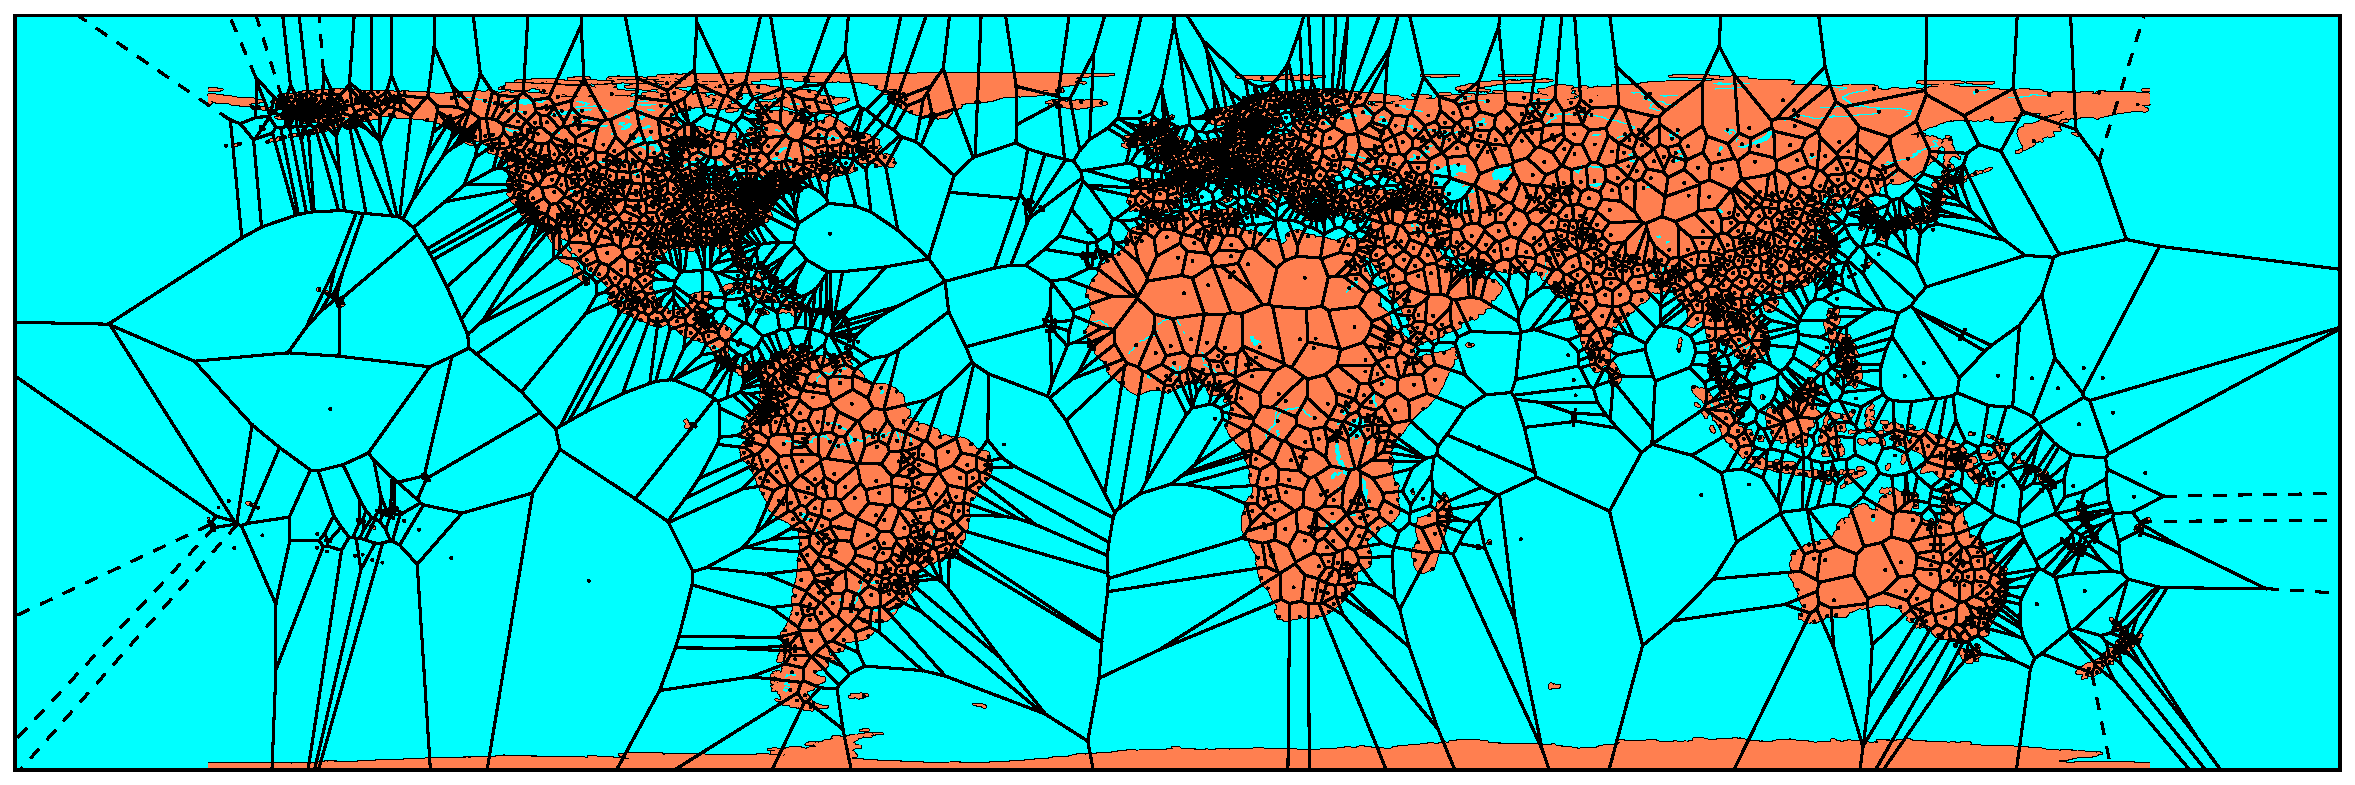
\includegraphics[width=1.0 \textwidth]{plots/voronoi.pdf}
	\caption{Voronoi tesselation based on airport locations. Airports are marked with a dot, region boundaries with lines and dashed lines.}
\end{figure}



\pagebreak
\appendix
\include{appendix}

\pagebreak
\printbibliography

\end{document}
